\documentclass[hidelinks]{ctexart}

\usepackage[sensei=潘海俊,gakka=電気力学,gakkabbr=ED]{styles/kurisu}
\usepackage{van-de-la-illinoise}

\begin{document}

\showtitle{電気力学}

\seclink{sec:sec1}{数学的基礎}
\seclink{sec:sec2}{電磁気学的基礎}
\seclink{sec:sec3}{静電場}
\seclink{sec:sec4}{静磁場}
\seclink{sec:sec5}{電磁波}
\clearpage
\phantomsection\label{sec:sec1}
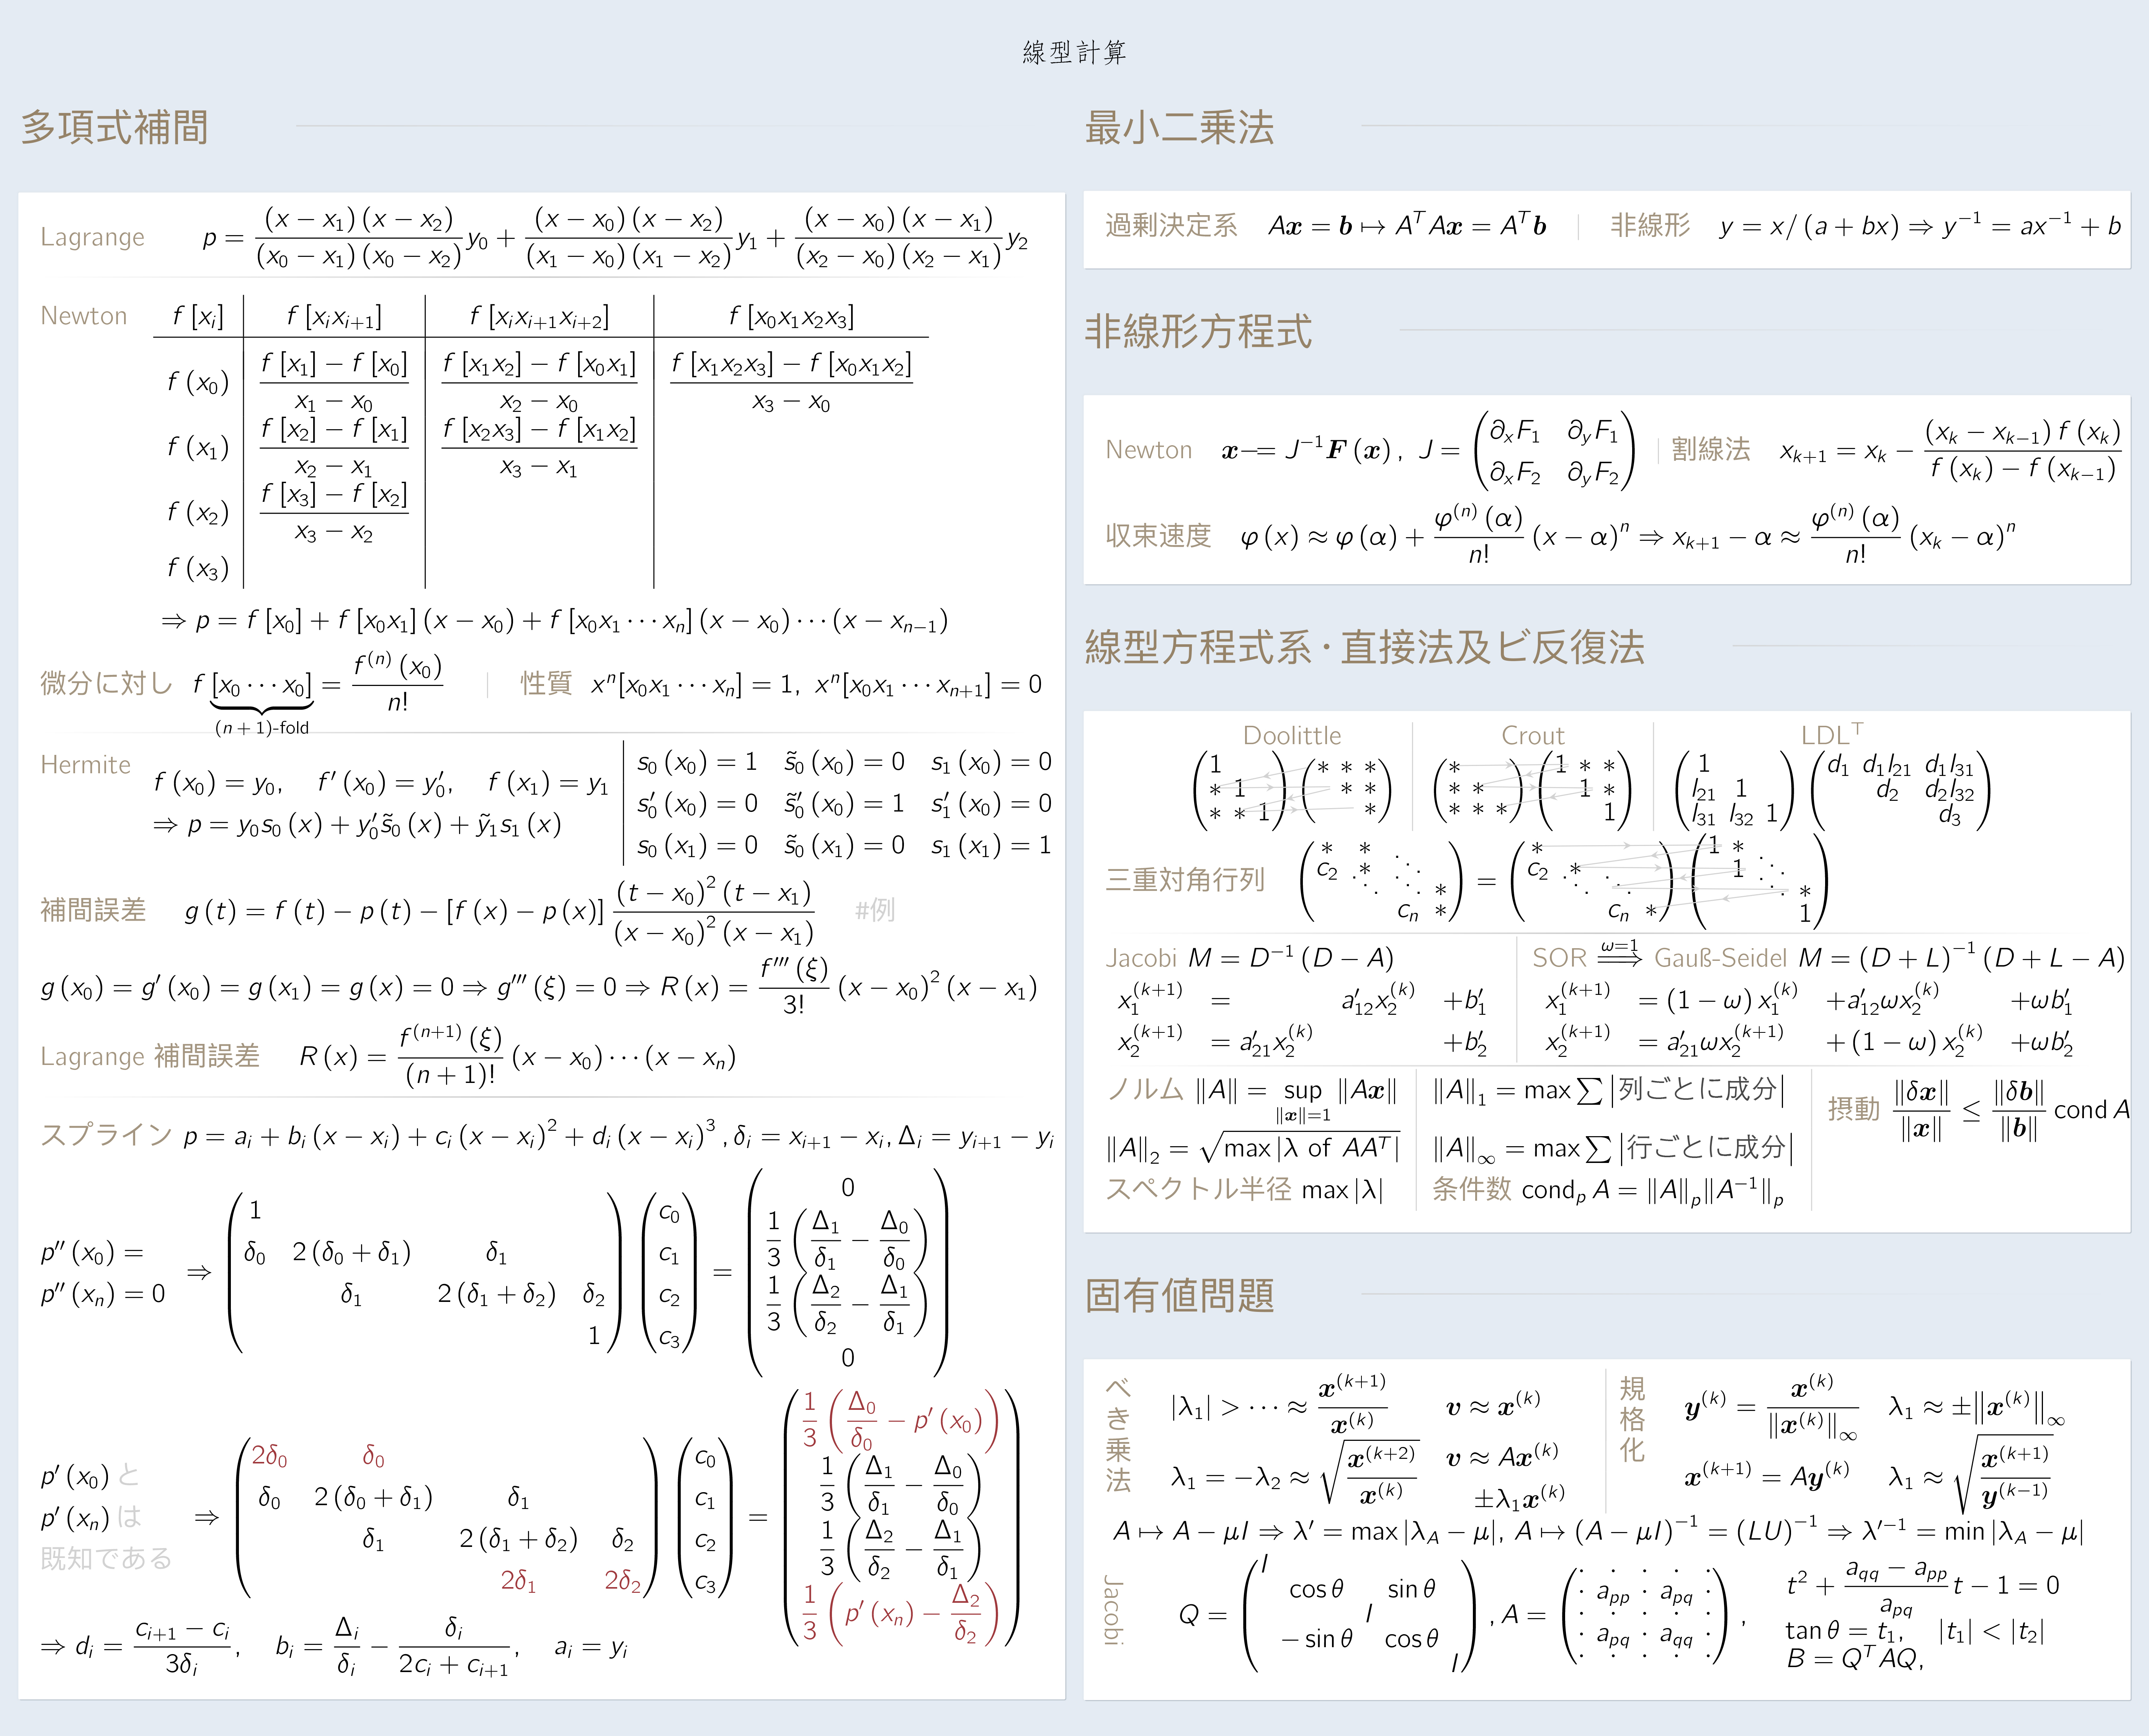
\includepdf[link,pages=-]{Elementary/Elementary.pdf}
\clearpage
\phantomsection\label{sec:sec2}
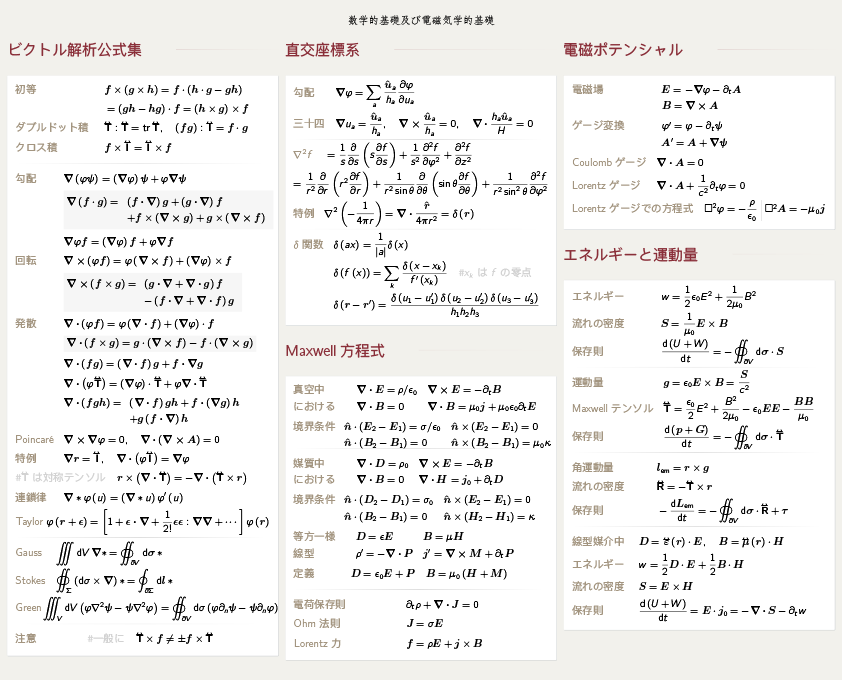
\includepdf[pages=-]{Fundamental/Fundamental.pdf}
\clearpage
\phantomsection\label{sec:sec3}
\includepdf[pages=-]{StaticElectricField/StaticElectricField.pdf}
\clearpage
\phantomsection\label{sec:sec4}
\includepdf[pages=-]{StaticMagneticField/StaticMagneticField.pdf}
\clearpage
\phantomsection\label{sec:sec3}
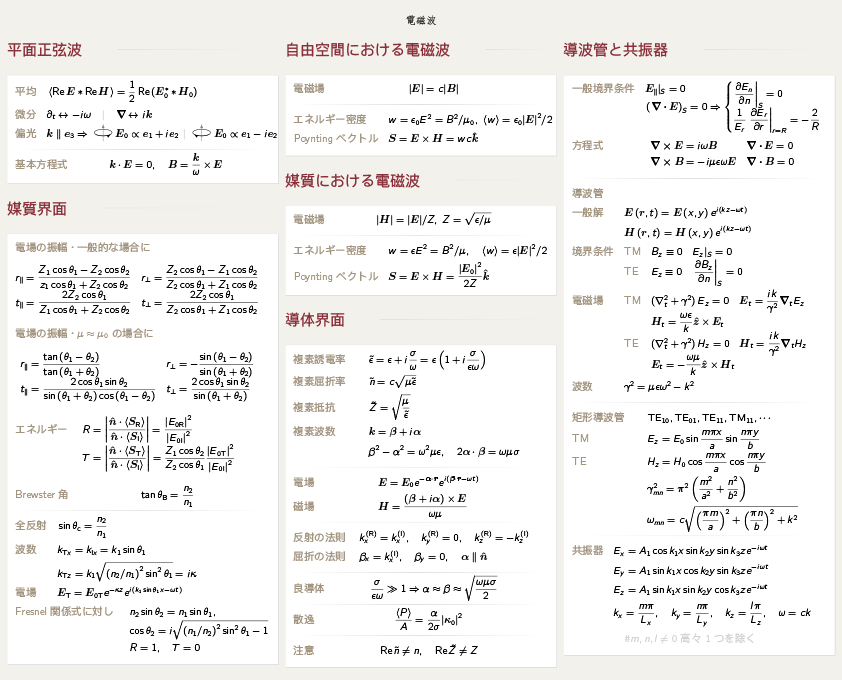
\includepdf[pages=-]{ElectromagneticWave/ElectromagneticWave.pdf}

\end{document}
